\section{Differentiability and sensitivity analysis}
\label{sec:gradient-calibration}

The tensor formulation permits reverse-mode automatic differentiation through
an unrolled SURF trajectory: for a scalar loss $\mathcal{J}$, derivatives can
be evaluated with respect to forcing components, initial states, and selected
parameters. For a loss depending on a time window, the backward pass returns
all control-variable derivatives at the cost of one reverse calculation,
rather than one additional forward integration per control, which is what
makes regional, multi-parameter process diagnosis and constrained parameter
estimation tractable. This section verifies the derivative
(Sect.~\ref{sec:gradient-verification}) and uses it for response diagnostics
(Sect.~\ref{sec:regional-response}); an initial-state retrieval against an
independently executed Fortran trajectory is provided in
Appendix~\ref{app:differentiability-support}, and the observation-space
application, identifiability, calibration, and structural attribution
against MODIS, follows in Sect.~\ref{sec:modis-evaluation}.

\subsection{Multi-step gradient verification}
\label{sec:gradient-verification}

Automatic differentiation must be verified independently before its
gradients are used to infer physical controls. A deterministic 24~h
idealized summer diurnal experiment with four identical land columns, hourly
coupling, no precipitation, and the complete autonomous SURF process
sequence provides three multi-step controls: a uniform air-temperature
forcing offset (loss: terminal mean skin temperature), a top-layer soil-water
initial-state offset (loss: terminal top-layer soil water), and the active
vegetation-class LAI table value (loss: 24~h accumulated evaporation). For
each control, the reverse-mode derivative was compared with a centred finite
difference over five perturbation magnitudes from $10^{-4}$ to $10^{-2}$.

Table~\ref{tab:gradient-verification} shows agreement better than
$4\times10^{-4}$ in relative error for all three derivatives; the residual
difference reflects the finite, fixed number of nonlinear surface-layer and
implicit-solver iterations in the discrete model, not a loss of gradient
connectivity (the perturbation-size dependence is shown in
Appendix~\ref{app:differentiability-support}). The test also identified an
inactive snow-throughfall division: tensor conditionals evaluate both
operands, so a snow-free and rain-free column can carry a masked $0/0$
division into the backward calculation despite a finite forward state. The
inactive denominator is replaced by one while the active path retains the
original expression, which leaves the forward solution unchanged and
prevents a nonphysical NaN derivative.

\begin{table}[t]
\caption{Verification of 24~h multi-step automatic-differentiation
derivatives against centred finite differences. The reported finite-difference
step is the value with the smallest relative discrepancy in the tested range.}
\label{tab:gradient-verification}
\centering
\small
\begin{tabular}{lrrr}
\hline
Control and loss & automatic derivative & relative error & $\epsilon$ \\
\hline
$\Delta T_{\rm air}\rightarrow \overline{T}_{\rm skin}^{24h}$ & $9.23691\times10^{-1}$ & $1.33\times10^{-5}$ & $10^{-2}$ K \\
$\Delta W_{\rm soil,1}^{0}\rightarrow \overline{W}_{\rm soil,1}^{24h}$ & $7.27416\times10^{-1}$ & $9.05\times10^{-5}$ & $3\times10^{-4}$ \\
$\mathrm{LAI}\rightarrow E_{\rm 24h}$ & $-3.51626\times10^{-1}$ & $3.66\times10^{-4}$ & $10^{-4}$ \\
\hline
\end{tabular}
\end{table}

\subsection{Regional and seasonal response diagnostics}
\label{sec:regional-response}

With no horizontal exchange in the standalone configuration, every column can
carry an independent infinitesimal air-temperature offset $\delta T_i$, and
the local terminal response
$S_i = \partial T_{{\rm skin},i}/\partial\delta T_i$ over a 6~h window of the
2018 CMFD forcing is obtained for all 97{,}709 columns from one forward
trajectory and one reverse pass; a centred-difference map would require one
perturbation integration per column. Figure~\ref{fig:regional-tair-sensitivity}
shows the spatial heterogeneity: the median response is
0.818~K~K$^{-1}$ (5th--95th percentiles 0.557--0.907~K~K$^{-1}$), so most
columns retain a locally smooth, sub-unity skin-temperature response. A small
set of columns (0.192~\% in this window) exceeds $1.5$~K~K$^{-1}$ in
magnitude; these sit near threshold-sensitive surface-layer, saturation, or
snow-regime states, are displayed explicitly rather than hidden by the
clipped colour scale, and mark where a derivative is a local linearization
rather than a finite-amplitude sensitivity.

Repeating the calculation at day-90, 180, 270, and 360 states of the annual
integration, after a 24~h unperturbed re-equilibration of the fast variables,
resolves the seasonal modulation
(Table~\ref{tab:seasonal-tair-response}). The median response ranges from
0.740~K~K$^{-1}$ in late June to 0.843~K~K$^{-1}$ in late December; summer
has both the broadest distribution and the largest fraction of
threshold-sensitive columns (4.17~\%), winter the most coherent response and
the smallest fraction (0.19~\%). The seasonal maps are provided in
Appendix~\ref{app:differentiability-support}. This separation between a
typical smooth process response and a small threshold-dominated set is a
property of the original parameterization, inherited rather than introduced
by the translation, and is carried into the interpretation of every gradient
result below.

\begin{figure}[t]
\centering
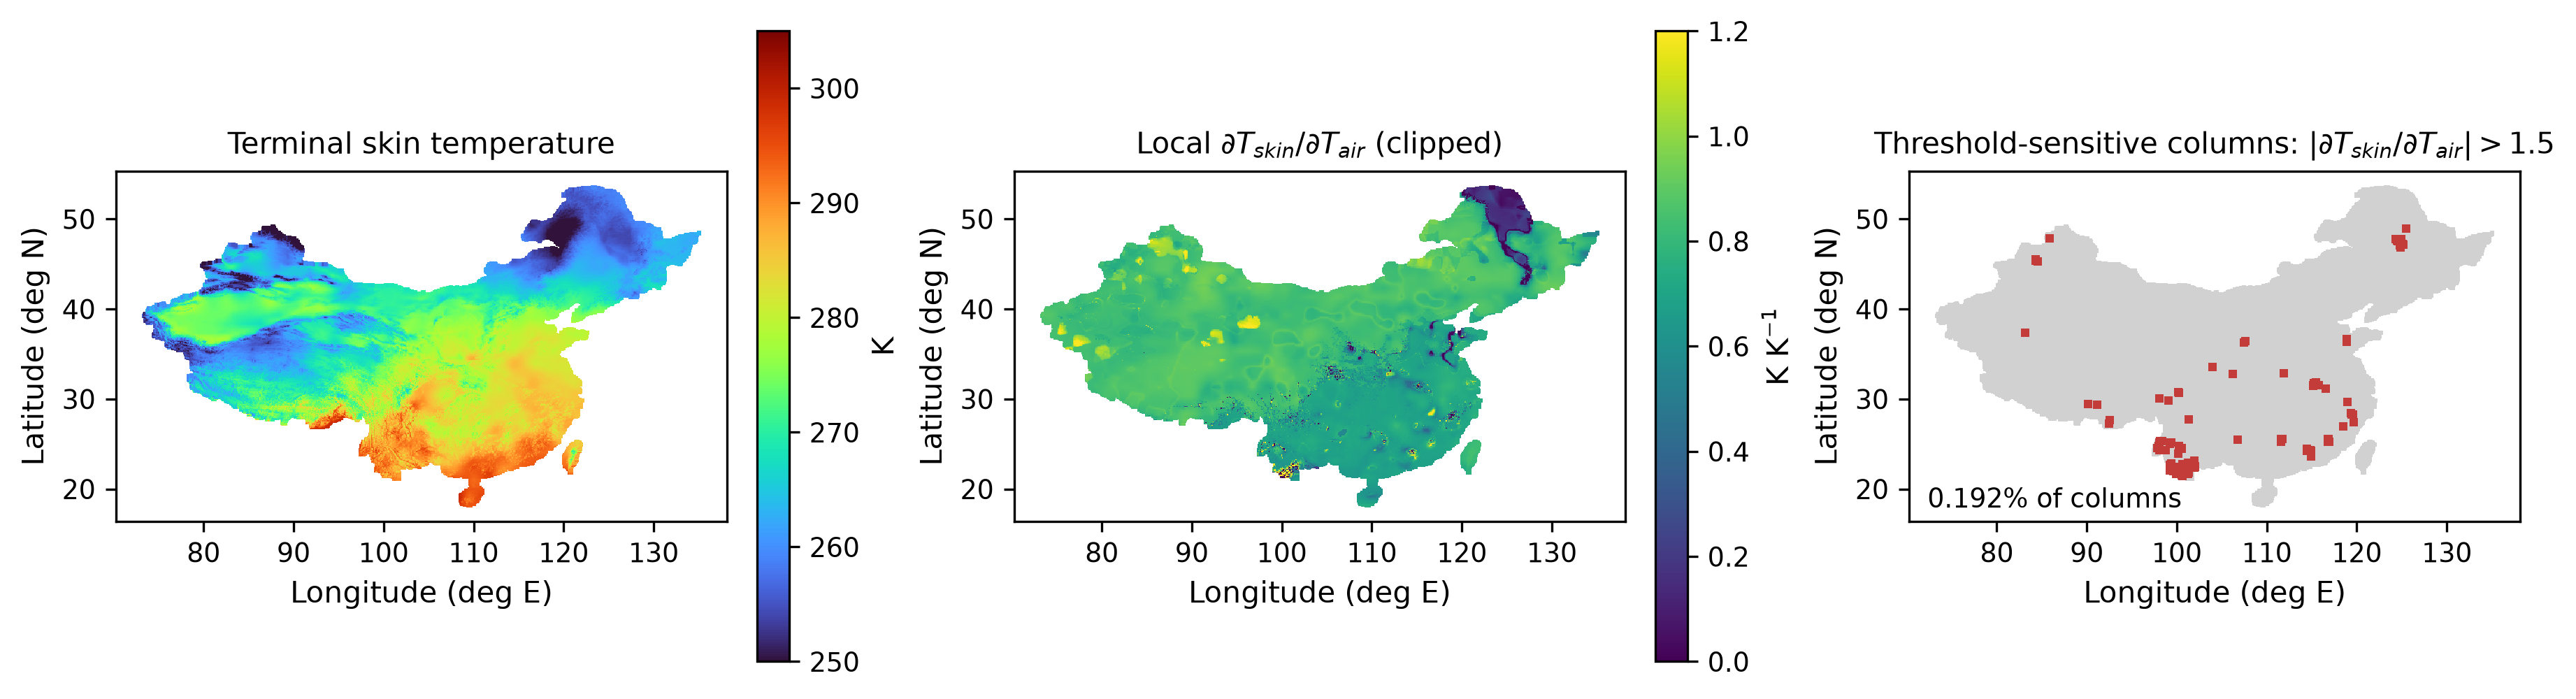
\includegraphics[width=\linewidth]{figures/regional_tair_sensitivity_maps.png}
\caption{Six-hour regional automatic-differentiation diagnostic under the
first 2018 CMFD forcing window from the common restart. Left: terminal
grid-mean skin temperature.
Centre: local response of terminal skin temperature to an independent
near-surface air-temperature offset at each column; the scale is clipped only
for visibility. Right: columns whose un-clipped absolute response exceeds
1.5~K~K$^{-1}$.}
\label{fig:regional-tair-sensitivity}
\end{figure}

\begin{table}[t]
\caption{Seasonal 6~h local air-temperature response of terminal skin
temperature over 97,709 CMFD land columns. The response is
$S_i=\partial T_{{\rm skin},i}/\partial T_{{\rm air},i}$. Threshold-sensitive
columns satisfy $|S_i|>1.5$~K~K$^{-1}$.}
\label{tab:seasonal-tair-response}
\centering
\small
\begin{tabular}{lrrr}
\hline
Sample & median (K K$^{-1}$) & 5th--95th percentile (K K$^{-1}$) & threshold-sensitive (\%) \\
\hline
Late March & 0.794 & 0.517--0.913 & 1.43 \\
Late June & 0.740 & 0.388--0.957 & 4.17 \\
Late September & 0.742 & 0.612--0.896 & 1.12 \\
Late December & 0.843 & 0.683--0.976 & 0.19 \\
\hline
\end{tabular}
\end{table}

\subsection{Interpretation and use of gradients}
\label{sec:gradient-interpretation}

The differentiable calculation retains the discrete physical regimes of the
reference scheme rather than smoothing them, following the formulation of
Sect.~\ref{sec:tensor-formulation}. Rain--snow partitioning, tile activation,
saturation bounds, and snow-cover clipping are
conditional statements, so the scheme is piecewise differentiable rather than
smooth. A derivative is therefore local to the active regime, is a one-sided
derivative at a regime crossing, and can be zero when a variable is limited
by a bound or does not enter the selected process pathway, behaviour that
reappears as the structurally zero and collinear control directions of
Appendix~\ref{app:modis-calibration} and is reported wherever gradient results
are interpreted. Potential calibration parameters include soil hydraulic
properties, snow albedo and density parameters, roughness-length scalings,
and canopy storage parameters; the verified multi-step derivative developed
here is the numerical foundation of the observation-space workflow of
Sect.~\ref{sec:modis-evaluation}.
